\documentclass[10pt,a4paper]{article}
\usepackage[utf8]{inputenc}
\usepackage{amsmath}
\usepackage{amsfonts}
\usepackage{amssymb}
\usepackage{graphicx}
\usepackage{float}
\usepackage[spaces,hyphens]{url}
\usepackage[colorlinks,allcolors=blue]{hyperref} 
\title{Project Notes}
\begin{document}
\maketitle

\section*{LISA Verification Binaries}
The Laser Interferometer Space Antenna(LISA) will be the first gravitational wave observatory in space. LISA will be operating in the low frequency part of the gravitational wave spectrum($10^4$-1 Hz). In this range, we expect to observe lots of ultracompact binaries with orbital periods shorter than few hours. Out of these UCBs, AM CVn type binaries are of particular interest. Due to therir strong GW signals, they are guaranteed to be  detetcted on LISA band. These are termed 'verification binaries'.

\section*{LISA Response Function}
From section 3.1 of \cite{cornish}, we get the varying portion for the round trip to be,

\begin{equation}
\delta l(t_2) = \frac{L sin^2 \theta}{2} \ \tau(cos \theta,f) \left[ h_{+}(t_2) cos 2\psi + h_{x}(t_2) sin 2\psi \right]
\end{equation}
Where, we have considered the arm to be in the x-z plane $ \textbf{u} = \hat{x} \ sin \theta + \hat{z} \ cos \theta$ \\


$\psi$ is the polarisation angle. $\tau$ is the transfer function as defined in eq(7) of \cite{cornish}

Now from we consider the plus and cross polarisation amplitudes of a binary black hole with an angle of inclination $i$ with the line of sight $\hat{z}$ (3.27a and 3.27b) of \cite{whelan}

We can then write,

\begin{equation}
h(t) = \frac{A(t)}{d}\ \left[ F_{+} \ \frac{1+ cos^2 i}{2} cos\Phi(t) + F_{\times} \ cosi \ sin\Phi(t) \right]
\end{equation}

Where the $F_{+} and F_{x}$ are the antenna response functions

In the present case we can write 

\begin{align}
\delta l&=\frac{A(t) L sin^2 \theta \tau(cos \theta,f)}{2d} \left[\frac{1+cos^2 i}{2} \ cos 2\psi \ cos \Phi(t) + cos i \ sin 2\psi \ sin \Phi(t)\right]\\
&=\frac{A(t) L sin^2 \theta \tau(cos \theta,f)}{2d} \left( \sqrt{ \frac{(1+cos^2 i)^2}{4} cos^2 2\psi  + cos^2 i sin^2 2\psi} \right)cos(\Phi(t)-\Psi)
\end{align}


The general formula is given by eq(8) of \cite{cornish}

FOr a general $\hat{\Omega}$ specified by $\theta,\omega$ in spherical coordinate system, we find that the antenna pattern becomes:

\begin{align}
F_{+}(\theta,\phi,\psi,i)&=\frac{(1+cos^2 i)}{2} \left[\frac{1}{2}(1+ cos^2 \theta) cos2\phi cos\psi - cos\theta sin2\phi sin2\psi \right]\\
F_{\times}(\theta,\phi,\psi,i)&=cos i \left[\frac{1}{2}(1+ cos^2 \theta) cos2\phi cos\psi + cos\theta sin2\phi cos2\psi \right]\\ 
\end{align}

If we put back $\theta=0$ and $\phi=0$ in [5] and [6] we get back the responses in eq [4].

The measured strain will be (as from eq 14 and 15)

\begin{align}
s&=\frac{\delta l_u (t) - \delta l_v (t)}{l}\\
&=\textbf{D}(\hat{\Omega},f) : h(\hat{\Omega},f,x,t)
\end{align}

where $D(\hat{\Omega},f) = \frac{1}{2}\left((u \otimes u) \tau - (v \otimes v) \tau \right)$

Depending on the orientation of the two arms specified by the u and v vector we get the final response as a function of the arm orientation,the orientation and location of binary.


\section*{HP Lib Verfication Binary}

We are interested in providing an independent prediction for $i$ and $\Psi$ for the AM CVn binary HP Lib. The binary consist of of on high mass white dwarf and a low mass star(brown dwarf).\\

\begin{table}[H]
\centering
\begin{tabular}{|c|c|c|c|}
\hline 
\rule[-1ex]{0pt}{2.5ex} Source & m1($M_{\odot}$) & m2($M_{\odot}$) & $P_{orb}$(sec) \\ 
\hline 
\rule[-1ex]{0pt}{2.5ex} HP Lib & 0.49-0.80 & 0.048-0.08 & 1102.70 \\ 
\hline 
\end{tabular}
\caption{The estimated values of mass and time period of HP Lib}
\end{table}

\begin{figure}
\centering
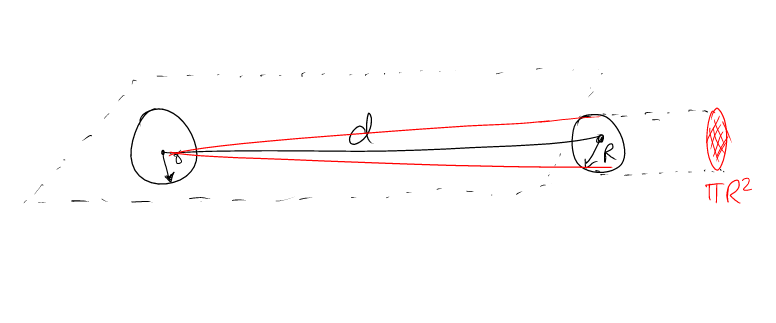
\includegraphics[scale=0.5]{diagram1.png}
\label{1}
\caption{The binary system HP Lib}
\end{figure}

Consider the verification binary HP Lib with masses $m_1$ and $m_2$ and period P \ref{1}. We can find the fraction of light recieved by the brown dwarf $m_2$ in the following way:

The flux from mass $m1$ obeys the inverse square law. Assuming a luminosity L, the flux at a distance d is given by $L/4 \pi d^2$. The cross section area for brown dwarf is $\pi R^2$.


Therefore, the total flux recieved is: $$\frac{L}{4 \pi d^2} \ \pi R^2 = \frac{L}{4} \ \left(\frac{R}{d}\right)^2 $$ where R is the radius of the brown dwarf and d is the seperation.

We can estimate d from the time period of the orbit. We know from Kepler's 3rd law that, $T^2 = \frac{4 \pi^{2}}{G (m_1 + m_2)} d^3$. We will denote $M=m_1 + m_2$

\begin{align*}
\frac{d}{c}&=\left(\frac{GM}{c^3}\right)^{1/3} \frac{T^{2/3}}{(4 \pi^{2})^{1/3}}\\
&=\frac{\left(\frac{GM}{c^3}\right)^{1/3}}{\left(\frac{GM_{\odot}}{c^3}\right)^{1/3}} \frac{T^{2/3}}{(4\pi^2)^{1/3}} (5 \times 10^{-6})^{1/3}
\end{align*}

Now the fraction of the light recieved is,

\begin{equation}
\frac{1}{4} \left(\frac{R}{c}\right)^2 \left(\frac{M}{M_{\odot}}\right)^{-2/3} \frac{T^{-4/3}}{(4 \pi^2)^{-2/3}} (5 \times 10^{-6})^{-2/3}
\end{equation}

For the first estimate, we can take $R/c \approx 0.1$ which if we subtitute above give an estimate of the light received to be 0.01315 

\begin{thebibliography}{9}

\bibitem{cornish}				\url{https://arxiv.org/pdf/gr-qc/0103075.pdf}

\bibitem{whelan} \url{https://dcc.ligo.org/public/0106/T1300666/003/Whelan_notes.pdf}
\end{thebibliography}

\end{document}